68. Построим каждую из прямых по двум точкам, отмеченным на рисунке (они найдены как точки пересечения данных прямых).
$$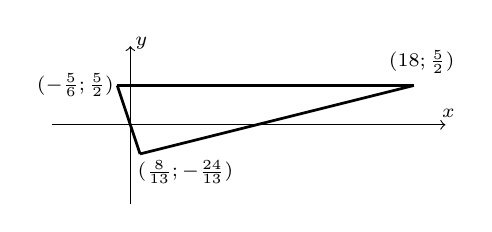
\begin{tikzpicture}[scale=0.2]
\tikzset {line01/.style={line width =0.5pt}}
\tikzset{line02/.style={line width =1pt}}
\tikzset{line03/.style={dashed,line width =0.5pt}}
%\filldraw [black] (0,0) circle (1pt);
\draw [->] (-5,0) -- (20,0);
\draw [->] (0,-5) -- (0,5);
\draw[line02] (18,2.5) -- (-0.833,2.5);
\draw[line02] (18,2.5) -- (0.615,-1.846);
\draw[line02] (0.615,-1.846) -- (-0.833,2.5);
\draw (20.2,0.7) node {\scriptsize $x$};
\draw (-3.5,2.5) node {\scriptsize $(-\frac{5}{6};\frac{5}{2})$};
\draw (3.5,-3) node {\scriptsize $(\frac{8}{13};-\frac{24}{13})$};
\draw (18.5,4) node {\scriptsize $(18;\frac{5}{2})$};
\draw (0.7,5.2) node {\scriptsize $y$};
\end{tikzpicture}$$
